% === Begin Label Data ===
% ID: 851
% 难度星级: 
% 标签: 
% 备注: 
% 组卷引用次数: 0
% === End  Label Data ===

\begin{problem}{2019}{G}{浙江卷}{9}{函数}
设 $ a $，$ b\in\mathbb{R} $，函数 $ f(x)=\begin{cases}
x,\,x<0,\\
\dfrac{1}{3}x^{3}-\dfrac{1}{2}(a+1)x^{2}+ax,\,x\geq0.
\end{cases} $ 若函数 $ y=f(x)-ax-b $ 恰有 3 个零点，则（\hspace{1cm}） (\hspace{1cm})
\begin{choices}
\choice{{$a<-1$，$b<0$}}
\choice{{$a<-1$，$b>0$}}
\choice{{$a>-1$，$b<0$}}
\choice{{$a>-1$，$b>0$}}
\end{choices}
\end{problem}

\begin{answer}
C
\end{answer}

\begin{solutions}
当 $ x<0 $ 时，$ y=f(x)-ax-b=x-ax-b=(1-a)x-b=0 $，得 $ x=\dfrac{b}{1-a} $；$ y=f(x)-ax-b $ 最多一个零点；

当 $ x\geq0 $ 时，$ y=f(x)-ax-b=\dfrac{1}{3}x^{3}-\dfrac{1}{2}(a+1)x^{2}+ax-ax-b=\dfrac{1}{3}x^{3}-\dfrac{1}{2}(a+1)x^{2}-b $，$ y'=x^{2}-(a+1)x $，

当 $ a+1\leq0 $，即 $ a\leq-1 $ 时，$ y'\geq0 $，$ y=f(x)-ax-b $ 在 $ [0,+\infty) $ 上递增，$ y=f(x)-ax-b $ 最多一个零点．不合题意；

当 $ a+1>0 $，即 $ a>-1 $ 时，令 $ y'>0 $ 得 $ x\in[a+1,+\infty) $，函数递增，令 $ y'<0 $ 得 $ x\in[0,a+1) $，函数递减；函数最多有 2 个零点；

根据题意函数 $ y=f(x)-ax-b $ 恰有 3 个零点 $ \Leftrightarrow $ 数 $ y=f(x)-ax-b $ 在 $ (-\infty,0) $ 上有一个零点，在 $ [0,+\infty) $ 上有 2 个零点，

如图：$ \therefore \dfrac{b}{1-a}<0 $ 且 $ \begin{cases}
-b>0\\
\dfrac{1}{3}(a+1)^{3}-\dfrac{1}{2}(a+1)(a+1)^{2}-b<0
\end{cases} $，

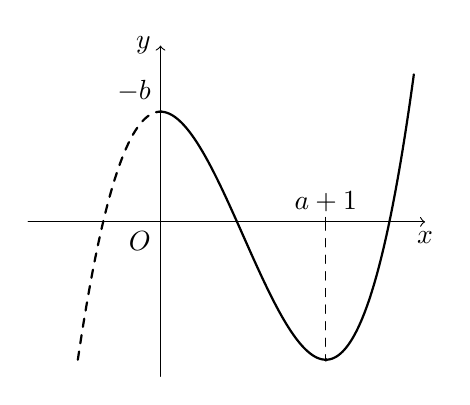
\begin{tikzpicture}[line cap=round,line join=round,scale=0.7]
\usetikzlibrary{calc,decorations.pathreplacing}

% 取参数（只用于定位；标签仍显示 -b、a+1）
\def\a{2.0}     % a>1
\def\b{-1.0}    % b<0

% 三次函数：g(x)=1/3 x^3 - 1/2(a+1)x^2 - b（把它在 x<0 处仅作“延拓示意”用虚线画）
\pgfmathsetmacro{\apone}{\a+1}
\pgfmathsetmacro{\yb}{-\b} % -b 的数值（b<0 时为正）

% 关键点：x=0 为极大点，x=a+1 为极小点
\pgfmathsetmacro{\ymax}{(1/3)*0^3 - (1/2)*(\apone)*0^2 - \b} % = -b
\pgfmathsetmacro{\ymin}{(1/3)*(\apone)^3 - (1/2)*(\apone)*(\apone)^2 - \b} % = -(a+1)^3/6 - b

% 坐标轴
\draw[->] (-2.4,0) -- (4.8,0) node[below] {$x$};
\draw[->] (0,-2.8) -- (0,3.2) node[left] {$y$};
\node[below left] at (0,0) {$O$};

% y 轴注记 -b（在 (0,-b) 处打刻度）
\draw (-0.08,\yb+1) -- (0.08,\yb+1);
\node[above left] at (0,\yb +1) {$-b$};

% x 轴注记 a+1（在 x=a+1 处打刻度）
\draw (\apone,-0.08) -- (\apone,0.08);
\node[above] at (\apone,0) {$a+1$};

% 画同一条三次曲线：x<0 虚线，x>=0 实线
\draw[dashed,thick,smooth,samples=180,domain=-1.5:0]
  plot (\x,{(1/3)*(\x)^3 - (1/2)*(\apone)*(\x)^2 - \b +1});
\draw[thick,smooth,samples=260,domain=0:4.6]
  plot (\x,{(1/3)*(\x)^3 - (1/2)*(\apone)*(\x)^2 - \b +1});

% 标出极小点处的虚线竖线（题图里那条）
\draw[dashed] (\apone,0) -- (\apone,\ymin+1);

% 点（可选：更像原图）
\fill (0,\ymax+1) circle (1.0pt);
\fill (\apone,\ymin+1) circle (1.0pt);

\end{tikzpicture}

解得 $ b<0 $，$ 1-a>0 $，$ b>-\dfrac{1}{6}(a+1)^{3} $．故选 C．
\end{solutions}